\subsection{Nullable class field values}
\label{subsec:library_of_transformations:instance_level_transformations:nullable_class_field_values}

\begin{figure}
    \centering
    \begin{subfigure}{0.95\textwidth}
        \centering
        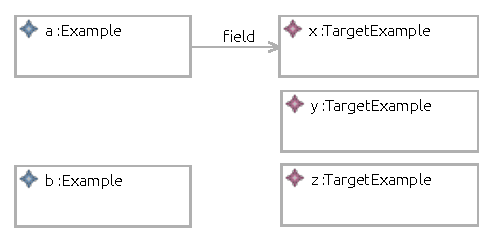
\includegraphics{images/05_library_of_transformations/03_instance_level_transformations/08_nullable_class_field_values/nullable_class_field_value.pdf}
        \caption{$Im_{NullableClassField}$ with examples of different nodes with different values for $\type{field}$}
        \label{fig:library_of_transformations:instance_level_transformations:nullable_class_field_values:visualisation:ecore}
    \end{subfigure}
    \\
    \begin{subfigure}{0.95\textwidth}
        \centering
        % To use this figure in your LaTeX document
% import the package groove/resources/groove2tikz.sty
%
\begin{tikzpicture}[scale=\tikzscale,name prefix=start-]
\node[basic_node] (n0) at (1.795, -0.405) {\ml{\uline{\textit{a}} : \textbf{Example}}};
\node[basic_node] (n1) at (1.795, -0.805) {\ml{\uline{\textit{b}} : \textbf{Example}}};
\node[basic_node] (n2) at (3.750, -0.440) {\ml{\uline{\textit{x}} : \textbf{TargetExample}}};
\node[basic_node] (n3) at (3.745, -0.815) {\ml{\uline{\textit{y}} : \textbf{TargetExample}}};
\node[basic_node] (n4) at (3.740, -1.205) {\ml{\uline{\textit{z}} : \textbf{TargetExample}}};

\path[basic_edge](n0.east |- 3.750, -0.440) -- node[lab] {\ml{field}} (n2) ;
\end{tikzpicture}

        \caption{$IG_{NullableClassField}$ with examples of different nodes with different values for $\type{field}$}
        \label{fig:library_of_transformations:instance_level_transformations:nullable_class_field_values:visualisation:groove}
    \end{subfigure}
    \caption{Visualisation of the transformation of field values from fields typed by nullable class types}
    \label{fig:library_of_transformations:instance_level_transformations:nullable_class_field_values:visualisation}
\end{figure}

This section introduces the instance level transformation belonging to the transformation of a nullable class field. The type level transformation for nullable class fields can be found in \cref{subsec:library_of_transformations:type_level_transformations:nullable_class_fields}. On the instance level, values for these fields are introduced.

\begin{defin}[Instance model $Im_{NullableClassField}$]
\label{defin:library_of_transformations:instance_level_transformations:nullable_class_field_values:imod_nullable_class_field}
Let $Im_{NullableClassField}$ be an instance model typed by $Tm_{NullableClassField}$ (\cref{defin:library_of_transformations:type_level_transformations:nullable_class_fields:tmod_nullable_class_field}). Define disjoint sets $valobjects$ and $nilobjects$. The objects in $valobjects$ will get a proper class value for the field introduced by $Tm_{NullableClassField}$, while the objects in $nilobjects$ get a $\type{nil}$ value for the same field. Furthermore, define a function $obids$ which maps each of these objects to their corresponding identifier and a function $values$, which maps the objects in $valobjects$ to its value for the field introduced by $Tm_{NullableClassField}$. $Im_{NullableClassField}$ is defined as:
\begin{align*}
Object =\ &nilobjects \cup valobjects \cup \{ values(ob) \mid ob \in valobjects \} \\
\mathrm{ObjectClass} =\ & \begin{cases}
    (ob, classtype) & \mathrm{if }\ ob \in nilobjects \cup valobjects\\
    (ob, fieldtype) & \mathrm{if }\ ob \in \{ values(ob) \mid ob \in valobjects \}
\end{cases}\\
\mathrm{ObjectId} =\ & \begin{cases}
    (ob, obids(ob)) & \mathrm{if }\ ob \in objects
\end{cases}\\
\mathrm{FieldValue} =\ & \begin{cases}
    ((ob, (classtype, name)), \type{nil}) & \mathrm{if }\ ob \in nilobjects\\
    ((ob, (classtype, name)), [\type{obj}, values(ob)]) & \mathrm{if }\ ob \in valobjects
\end{cases} \\
\mathrm{DefaultValue} =\ & \{\}
\end{align*}
\isabellelref{imod_nullable_class_field}{Ecore-GROOVE-Mapping-Library.NullableClassFieldValue}
\end{defin}

\begin{thm}[Correctness of $Im_{NullableClassField}$]
\label{defin:library_of_transformations:instance_level_transformations:nullable_class_field_values:imod_nullable_class_field_correct}
$Im_{NullableClassField}$ (\cref{defin:library_of_transformations:instance_level_transformations:nullable_class_field_values:imod_nullable_class_field}) is a valid instance model in the sense of \cref{defin:formalisations:ecore_formalisation:instance_models:model_validity}.
\isabellelref{imod_nullable_class_field_correct}{Ecore-GROOVE-Mapping-Library.NullableClassFieldValue}
\end{thm}

A visual representation of $Im_{NullableClassField}$ with $valobjects = \{ob_a\}$ and $nilobjects = \{ob_b\}$ can be seen in \cref{fig:library_of_transformations:instance_level_transformations:nullable_class_field_values:visualisation:ecore}. In this visualisation, the field value for $ob_a$ is defined as $values(ob_a) = ob_x$. Furthermore, the value for $ob_b$ is $\type{nil}$, because it occurs within the set $nilobjects$. Like the previous transformations for field values, the value needs to be set for all objects that are typed by the class type corresponding to the field. Failing to do so would result in an invalid instance model after it is combined with another model, as the next definition will show. The correctness proof of $Im_{NullableClassField}$ only is already quite involved, but not be included here for conciseness. It can be found as part of the validated Isabelle proofs.

In order to make composing transformation functions possible, $Im_{NullableClassField}$ should be compatible with the instance model it is combined with.

\begin{thm}[Correctness of $\mathrm{combine}(Im, Im_{NullableClassField})$]
\label{defin:library_of_transformations:instance_level_transformations:nullable_class_field_values:imod_nullable_class_field_combine_correct}
Assume an instance model $Im$ that is valid in the sense of \cref{defin:formalisations:ecore_formalisation:instance_models:model_validity}. Then $Im$ is compatible with $Im_{NullableClassField}$ (in the sense of \cref{defin:transformation_framework:instance_models_and_instance_graphs:combining_instance_models:compatibility}) if:
\begin{itemize}
    \item All requirements of \cref{defin:library_of_transformations:type_level_transformations:nullable_class_fields:tmod_nullable_class_field_combine_correct} are met, to ensure the combination of the corresponding type models is valid;
    \item The class type on which the field is defined by $Tm_{NullableClassField}$ may not be extended by another class type in the type model corresponding to $Im$;
    \item All of the objects in the sets $nilobjects$ and $valobjects$ must already be objects in $Im$;
    \item All of the objects referenced by the objects in the set $valobjects$ must already be objects in $Im$;
    \item All objects typed by the class type on which the field is defined must occur in the set $nilobjects \cup valobjects$ and thus have a value in $Im_{NullableClassField}$;
    \item For all of the objects in the set $objects$, the identifier set by $obids$ must be the same identifier as set by $Im$ for that object;
    \item The sets $valobjects$ and $nilobjects$ must be disjoint, each object only gets a proper class value or a nil value, not both;
    \item For all objects in set $valobjects$, the value set by the $values$ function must be valid.
\end{itemize}
\isabellelref{imod_nullable_class_field_combine_correct}{Ecore-GROOVE-Mapping-Library.NullableClassFieldValue}
\end{thm}

\begin{proof}
Use \cref{defin:transformation_framework:instance_models_and_instance_graphs:combining_instance_models:imod_combine_merge_correct}. It is possible to show that all assumptions hold. Now we have shown that $\mathrm{combine}(Im, Im_{NullableClassField})$ is consistent in the sense of \cref{defin:formalisations:ecore_formalisation:instance_models:model_validity}.
\end{proof}

As explained earlier, $Im_{NullableClassField}$ needs to introduce values for all objects that are typed by the class type on which the field is defined. This is enforced by the requirements of \cref{defin:library_of_transformations:instance_level_transformations:nullable_class_field_values:imod_nullable_class_field_combine_correct}. The proof is not included here for conciseness, but can be found as part of the validated proofs in Isabelle.

The definitions and theorems for introducing values for fields of data types within Ecore are now complete. 

\subsubsection{Encoding as edges and nodes}

In the type level transformation of nullable class fields, nullable class fields were encoded in GROOVE as edge types to a corresponding encoded node type. On the instance level, this edge type will be used and edges will be created to give a value to each node type that has the field defined. The encoding corresponding to $Im_{NullableClassField}$ can then be represented as $IG_{NullableClassField}$, defined in the following definition:

\begin{defin}[Instance graph $IG_{NullableClassField}$]
\label{defin:library_of_transformations:instance_level_transformations:nullable_class_field_values:ig_nullable_class_field_as_edge_type}
Let $IG_{NullableClassField}$ be the instance graph typed by type graph $TG_{NullableClassField}$ (\cref{defin:library_of_transformations:type_level_transformations:nullable_class_fields:tg_nullable_class_field_as_edge_type}). Reuse the sets $nilobjects$ and $valobjects$ from $Im_{NullableClassField}$. Moreover, reuse the functions $obids$ and $values$ from $Im_{NullableClassField}$.

The objects in the sets $nilobjects$ and $valobjects$ are converted to nodes in $Im_{NullableClassField}$. For each of these objects, an edge of the encoded field is created. This edge targets a node that corresponds to the value set by $values$ for the corresponding object in $valobjects$. The outgoing multiplicity of the edge type created by $TG_{NullableClassField}$ is $0..1$, such that the objects in $nilobjects$ do not need to have this edge, representing the absence of a value. Finally, the identity of the objects is defined using $obids$. $IG_{NullableClassField}$ is defined as:
\begin{align*}
N =\ & nilobjects \cup valobjects \cup \{values(ob) \mid ob \in valobjects\} \\
E =\ & \big\{\big(ob, (\mathrm{ns\_\!to\_\!list}(classtype), \langle name \rangle, \mathrm{ns\_\!to\_\!list}(fieldtype)), values(ob)\big) \mid ob \in valobjects \big\} \\
\mathrm{ident} =\ & \begin{cases}
    (obids(ob), ob) & \mathrm{if }\ ob \in objects
\end{cases}
\end{align*}
with
\begin{align*}
\mathrm{type}_n =\ & \begin{cases}
    (ob, \mathrm{ns\_\!to\_\!list}(classtype)) & \mathrm{if }\ ob \in nilobjects \cup valobjects\\
    (ob, \mathrm{ns\_\!to\_\!list}(fieldtype)) & \mathrm{if }\ ob \in \{values(ob) \mid ob \in valobjects\}
\end{cases}
\end{align*}
\isabellelref{ig_nullable_class_field_as_edge_type}{Ecore-GROOVE-Mapping-Library.NullableClassFieldValue}
\end{defin}

\begin{thm}[Correctness of $IG_{NullableClassField}$]
\label{defin:library_of_transformations:instance_level_transformations:nullable_class_field_values:ig_nullable_class_field_as_edge_type_correct}
$IG_{NullableClassField}$ (\cref{defin:library_of_transformations:instance_level_transformations:nullable_class_field_values:ig_nullable_class_field_as_edge_type}) is a valid instance graph in the sense of \cref{defin:formalisations:groove_formalisation:instance_graphs:instance_graph_validity}.
\isabellelref{ig_nullable_class_field_as_edge_type_correct}{Ecore-GROOVE-Mapping-Library.NullableClassFieldValue}
\end{thm}

A visual representation of $IG_{NullableClassField}$ with $valobjects = \{ob_a\}$ and $nilobjects = \{ob_b\}$ can be seen in \cref{fig:library_of_transformations:instance_level_transformations:nullable_class_field_values:visualisation:groove}. Like the previous visualisation, the field value for $ob_a$ is defined as $values(ob_a) = ob_x$. Since $ob_b$ was in the set $nilobjects$, no edge has been created for this node. Like the previous field encodings, one needs to set the values for the field for all objects of the encoded class type at once. Failing to do so would result in an invalid instance graph after it is combined with another graph, as the next definition will show. The correctness proof of $IG_{NullableClassField}$ only is already quite involved, but not be included here for conciseness. It can be found as part of the validated Isabelle proofs.

In order to make composing transformation functions possible, $IG_{NullableClassField}$ should be compatible with the instance graph it is combined with.

\begin{thm}[Correctness of $\mathrm{combine}(IG, IG_{NullableClassField})$]
\label{defin:library_of_transformations:instance_level_transformations:nullable_class_field_values:ig_nullable_class_field_as_edge_type_combine_correct}
Assume an instance graph $IG$ that is valid in the sense of \cref{defin:formalisations:groove_formalisation:instance_graphs:instance_graph_validity}. Then $IG$ is compatible with $IG_{NullableClassField}$ (in the sense of \cref{defin:transformation_framework:instance_models_and_instance_graphs:combining_instance_graphs:compatibility}) if:
\begin{itemize}
    \item All requirements of \cref{defin:library_of_transformations:type_level_transformations:nullable_class_fields:tg_nullable_class_field_as_edge_type_combine_correct} are met, to ensure the combination of the corresponding type graphs is valid;
    \item The node type on which the corresponding field is defined is not extended by other node types within the type graph corresponding to $IG$;
    \item All nodes in $IG$ are also nodes in $IG_{NullableClassField}$;
    \item For all nodes shared between $IG$ and $IG_{NullableClassField}$, each node must have the same identifier in both $IG$ and $IG_{NullableClassField}$;
    \item The sets $valobjects$ and $nilobjects$ must be disjoint, each node gets either one edge to another node, or no edge at all;
    \item For all nodes for which the field is set, the $values$ function must define a valid value.
\end{itemize}
\isabellelref{ig_nullable_class_field_as_edge_type_combine_correct}{Ecore-GROOVE-Mapping-Library.NullableClassFieldValue}
\end{thm}

\begin{proof}
Use \cref{defin:transformation_framework:instance_models_and_instance_graphs:combining_instance_graphs:ig_combine_merge_correct}. It is possible to show that all assumptions hold. Now we have shown that $\mathrm{combine}(IG, IG_{NullableClassField})$ is valid in the sense of \cref{defin:formalisations:groove_formalisation:instance_graphs:instance_graph_validity}.
\end{proof}

The next definitions define the transformation function from $Im_{NullableClassField}$ to $IG_{NullableClassField}$:

\begin{defin}[Transformation function $f_{NullableClassField}$]
\label{defin:library_of_transformations:instance_level_transformations:nullable_class_field_values:imod_nullable_class_field_to_ig_nullable_class_field_as_edge_type}
The transformation function $f_{NullableClassField}(Im)$ is defined as:
\begin{align*}
N =\ & Object_{Im}  \\
E =\ & \big\{\big(ob, (\mathrm{ns\_\!to\_\!list}(classtype), \langle name \rangle, \mathrm{ns\_\!to\_\!list}(fieldtype)), values(ob)\big) \mid\\&ob \in Object_{Im} \land ob \in valobjects \big\} \\
\mathrm{ident} =\ & \begin{cases}
    (obids(ob), ob) & \mathrm{if }\ ob \in Object_{Im}
\end{cases}
\end{align*}
with
\begin{align*}
\mathrm{type}_n =\ & \begin{cases}
    (ob, \mathrm{ns\_\!to\_\!list}(name)) & \mathrm{if }\ ob \in Object_{Im} \land ob \in nilobjects \cup valobjects\\
    (ob, \mathrm{ns\_\!to\_\!list}(name)) & \mathrm{if }\ ob \in Object_{Im} \land ob \in \{values(ob) \mid ob \in valobjects\} 
\end{cases}
\end{align*}
\isabellelref{imod_nullable_class_field_to_ig_nullable_class_field_as_edge_type}{Ecore-GROOVE-Mapping-Library.NullableClassFieldValue}
\end{defin}

\begin{thm}[Correctness of $f_{NullableClassField}$]
\label{defin:library_of_transformations:instance_level_transformations:nullable_class_field_values:imod_nullable_class_field_to_ig_nullable_class_field_as_edge_type_func}
$f_{NullableClassField}(Im)$ (\cref{defin:library_of_transformations:instance_level_transformations:nullable_class_field_values:imod_nullable_class_field_to_ig_nullable_class_field_as_edge_type}) is a valid transformation function in the sense of \cref{defin:transformation_framework:instance_models_and_instance_graphs:combining_transformation_functions:transformation_function_instance_model_instance_graph} transforming $Im_{NullableClassField}$ into $IG_{NullableClassField}$.
\isabellelref{imod_nullable_class_field_to_ig_nullable_class_field_as_edge_type_func}{Ecore-GROOVE-Mapping-Library.NullableClassFieldValue}
\end{thm}

The proof of the correctness of $f_{NullableClassField}$ will not be included here. Instead, it can be found in the validated Isabelle theories.

Finally, to complete the transformation, the transformation function that transforms $IG_{NullableClassField}$ into $Im_{NullableClassField}$ is defined:

\begin{defin}[Transformation function $f'_{NullableClassField}$]
\label{defin:library_of_transformations:instance_level_transformations:nullable_class_field_values:ig_nullable_class_field_as_edge_type_to_imod_nullable_class_field}
The transformation function $f'_{NullableClassField}(IG)$ is defined as:
\begin{align*}
Object =\ &N_{IG} \\
\mathrm{ObjectClass} =\ & \begin{cases}
    (ob, classtype) & \mathrm{if }\ ob \in N_{IG} \land ob \in nilobjects \cup valobjects \\
    (ob, fieldtype) & \mathrm{if }\ ob \in N_{IG} \land ob \in \{values(ob) \mid ob \in valobjects\}
\end{cases}\\
\mathrm{ObjectId} =\ & \begin{cases}
    (ob, obids(ob)) & \mathrm{if }\ ob \in N_{IG}
\end{cases}\\
\mathrm{FieldValue} =\ & \begin{cases}
    ((ob, (classtype, name)), \type{nil}) & \mathrm{if }\ ob \in N_{IG} \land ob \in nilobjects\\
    ((ob, (classtype, name)), [\type{obj}, values(ob)]) & \mathrm{if }\ ob \in N_{IG} \land ob \in valobjects
\end{cases} \\
\mathrm{DefaultValue} =\ & \{\}
\end{align*}
\isabellelref{ig_nullable_class_field_as_edge_type_to_imod_nullable_class_field}{Ecore-GROOVE-Mapping-Library.NullableClassFieldValue}
\end{defin}

\begin{thm}[Correctness of $f'_{NullableClassField}$]
\label{defin:library_of_transformations:instance_level_transformations:nullable_class_field_values:ig_nullable_class_field_as_edge_type_to_tmod_class_func}
$f'_{NullableClassField}(IG)$ (\cref{defin:library_of_transformations:instance_level_transformations:nullable_class_field_values:ig_nullable_class_field_as_edge_type_to_imod_nullable_class_field}) is a valid transformation function in the sense of \cref{defin:transformation_framework:instance_models_and_instance_graphs:combining_transformation_functions:transformation_function_instance_graph_instance_model} transforming $IG_{NullableClassField}$ into $Im_{NullableClassField}$.
\isabellelref{ig_nullable_class_field_as_edge_type_to_imod_nullable_class_field_func}{Ecore-GROOVE-Mapping-Library.NullableClassFieldValue}
\end{thm}

Once more, the correctness proof is not included here but can be found in the validated Isabelle proofs of this thesis.